\documentclass{standalone}
\usepackage{tikz}
\usetikzlibrary{patterns, positioning}

\begin{document}
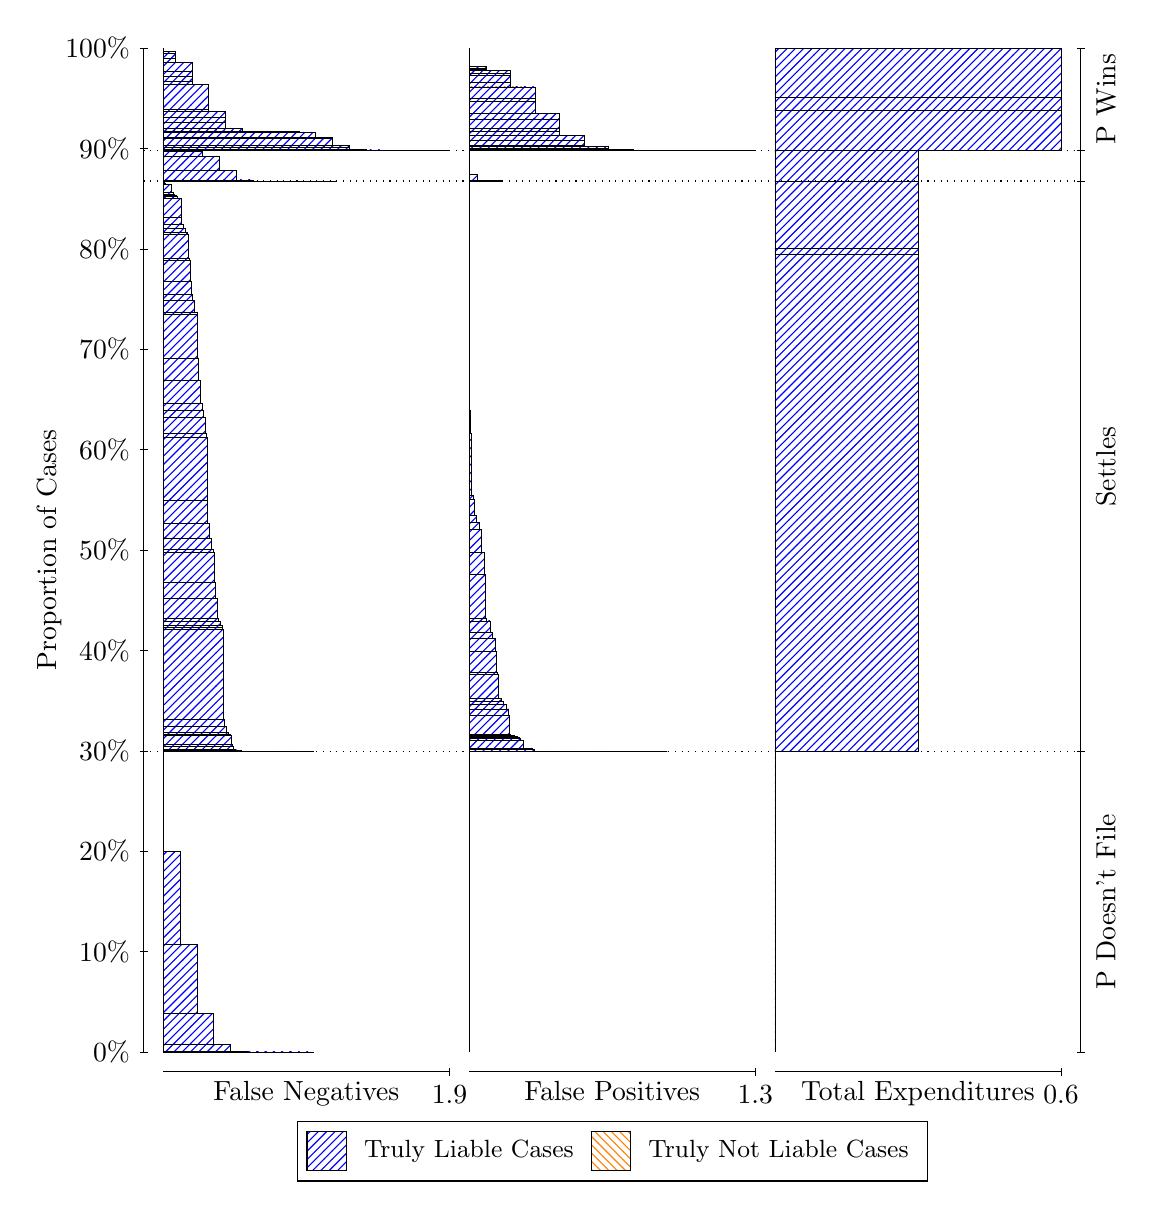
\begin{tikzpicture}
\draw[black, very thin] (1.5,1.75) -- (1.5,14.5);
\node[rotate=90, anchor=center] at (0.3, 8.125) {Proportion of Cases};
\draw[black, very thin] (1.45,1.75) -- (1.55,1.75);
\node[anchor=east] at (1.45, 1.75) {0\%};
\draw[black, very thin] (1.45,3.025) -- (1.55,3.025);
\node[anchor=east] at (1.45, 3.025) {10\%};
\draw[black, very thin] (1.45,4.3) -- (1.55,4.3);
\node[anchor=east] at (1.45, 4.3) {20\%};
\draw[black, very thin] (1.45,5.575) -- (1.55,5.575);
\node[anchor=east] at (1.45, 5.575) {30\%};
\draw[black, very thin] (1.45,6.85) -- (1.55,6.85);
\node[anchor=east] at (1.45, 6.85) {40\%};
\draw[black, very thin] (1.45,8.125) -- (1.55,8.125);
\node[anchor=east] at (1.45, 8.125) {50\%};
\draw[black, very thin] (1.45,9.4) -- (1.55,9.4);
\node[anchor=east] at (1.45, 9.4) {60\%};
\draw[black, very thin] (1.45,10.675) -- (1.55,10.675);
\node[anchor=east] at (1.45, 10.675) {70\%};
\draw[black, very thin] (1.45,11.95) -- (1.55,11.95);
\node[anchor=east] at (1.45, 11.95) {80\%};
\draw[black, very thin] (1.45,13.225) -- (1.55,13.225);
\node[anchor=east] at (1.45, 13.225) {90\%};
\draw[black, very thin] (1.45,14.5) -- (1.55,14.5);
\node[anchor=east] at (1.45, 14.5) {100\%};

\draw[black, very thin] (13.4,1.75) -- (13.4,14.5);
\draw[black, very thin] (13.35,1.75) -- (13.45,1.75);
\node[anchor=west] at (13.35, 1.75) {};
\draw[black, very thin] (13.35,5.563) -- (13.45,5.563);
\node[anchor=west] at (13.35, 5.563) {};
\draw[black, very thin] (13.35,12.811) -- (13.45,12.811);
\node[anchor=west] at (13.35, 12.811) {};
\draw[black, very thin] (13.35,13.204) -- (13.45,13.204);
\node[anchor=west] at (13.35, 13.204) {};
\draw[black, very thin] (13.35,14.5) -- (13.45,14.5);
\node[anchor=west] at (13.35, 14.5) {};

\draw[black, very thin, pattern color=blue, pattern=north east lines] (1.75,1.75) rectangle (3.6623,1.75);
\draw[black, very thin, pattern color=blue, pattern=north east lines] (1.75,1.75) rectangle (3.4498,1.75);
\draw[black, very thin, pattern color=blue, pattern=north east lines] (1.75,1.75) rectangle (3.2373,1.75);
\draw[black, very thin, pattern color=blue, pattern=north east lines] (1.75,1.75) rectangle (3.0249,1.7503);
\draw[black, very thin, pattern color=blue, pattern=north east lines] (1.75,1.7503) rectangle (2.8124,1.7582);
\draw[black, very thin, pattern color=blue, pattern=north east lines] (1.75,1.7582) rectangle (2.5999,1.8434);
\draw[black, very thin, pattern color=blue, pattern=north east lines] (1.75,1.8434) rectangle (2.3874,2.2366);
\draw[black, very thin, pattern color=blue, pattern=north east lines] (1.75,2.2366) rectangle (2.175,3.1157);
\draw[black, very thin, pattern color=blue, pattern=north east lines] (1.75,3.1157) rectangle (1.9625,4.2995);
\draw[black, very thin, pattern color=orange, pattern=north west lines] (1.75,4.2995) rectangle (1.75,4.2995);
\draw[black, very thin, pattern color=blue, pattern=north east lines] (1.75,4.2995) rectangle (1.75,5.563);
\draw[black, very thin, pattern color=blue, pattern=north east lines] (1.75,5.563) rectangle (3.6623,5.563);
\draw[black, very thin, pattern color=blue, pattern=north east lines] (1.75,5.563) rectangle (3.5667,5.563);
\draw[black, very thin, pattern color=blue, pattern=north east lines] (1.75,5.563) rectangle (3.4711,5.563);
\draw[black, very thin, pattern color=blue, pattern=north east lines] (1.75,5.563) rectangle (3.4498,5.563);
\draw[black, very thin, pattern color=blue, pattern=north east lines] (1.75,5.563) rectangle (3.3754,5.563);
\draw[black, very thin, pattern color=blue, pattern=north east lines] (1.75,5.563) rectangle (3.3542,5.563);
\draw[black, very thin, pattern color=blue, pattern=north east lines] (1.75,5.563) rectangle (3.2798,5.563);
\draw[black, very thin, pattern color=blue, pattern=north east lines] (1.75,5.563) rectangle (3.2586,5.563);
\draw[black, very thin, pattern color=blue, pattern=north east lines] (1.75,5.563) rectangle (3.2373,5.563);
\draw[black, very thin, pattern color=blue, pattern=north east lines] (1.75,5.563) rectangle (3.1842,5.563);
\draw[black, very thin, pattern color=blue, pattern=north east lines] (1.75,5.563) rectangle (3.163,5.563);
\draw[black, very thin, pattern color=blue, pattern=north east lines] (1.75,5.563) rectangle (3.1417,5.563);
\draw[black, very thin, pattern color=blue, pattern=north east lines] (1.75,5.563) rectangle (3.0886,5.563);
\draw[black, very thin, pattern color=blue, pattern=north east lines] (1.75,5.563) rectangle (3.0673,5.563);
\draw[black, very thin, pattern color=blue, pattern=north east lines] (1.75,5.563) rectangle (3.0461,5.563);
\draw[black, very thin, pattern color=blue, pattern=north east lines] (1.75,5.563) rectangle (3.0249,5.563);
\draw[black, very thin, pattern color=blue, pattern=north east lines] (1.75,5.563) rectangle (2.993,5.563);
\draw[black, very thin, pattern color=blue, pattern=north east lines] (1.75,5.563) rectangle (2.9717,5.5631);
\draw[black, very thin, pattern color=blue, pattern=north east lines] (1.75,5.5631) rectangle (2.9505,5.5631);
\draw[black, very thin, pattern color=blue, pattern=north east lines] (1.75,5.5631) rectangle (2.9292,5.5632);
\draw[black, very thin, pattern color=blue, pattern=north east lines] (1.75,5.5632) rectangle (2.8974,5.5636);
\draw[black, very thin, pattern color=blue, pattern=north east lines] (1.75,5.5636) rectangle (2.8761,5.5636);
\draw[black, very thin, pattern color=blue, pattern=north east lines] (1.75,5.5636) rectangle (2.8549,5.5645);
\draw[black, very thin, pattern color=blue, pattern=north east lines] (1.75,5.5645) rectangle (2.8336,5.5652);
\draw[black, very thin, pattern color=blue, pattern=north east lines] (1.75,5.5652) rectangle (2.8124,5.5653);
\draw[black, very thin, pattern color=blue, pattern=north east lines] (1.75,5.5653) rectangle (2.7805,5.5661);
\draw[black, very thin, pattern color=blue, pattern=north east lines] (1.75,5.5661) rectangle (2.7593,5.5709);
\draw[black, very thin, pattern color=blue, pattern=north east lines] (1.75,5.5709) rectangle (2.738,5.5764);
\draw[black, very thin, pattern color=blue, pattern=north east lines] (1.75,5.5764) rectangle (2.7168,5.5778);
\draw[black, very thin, pattern color=blue, pattern=north east lines] (1.75,5.5778) rectangle (2.7061,5.5789);
\draw[black, very thin, pattern color=blue, pattern=north east lines] (1.75,5.5789) rectangle (2.6849,5.5865);
\draw[black, very thin, pattern color=blue, pattern=north east lines] (1.75,5.5865) rectangle (2.6636,5.5885);
\draw[black, very thin, pattern color=blue, pattern=north east lines] (1.75,5.5885) rectangle (2.6424,5.6271);
\draw[black, very thin, pattern color=blue, pattern=north east lines] (1.75,5.6271) rectangle (2.6212,5.6546);
\draw[black, very thin, pattern color=blue, pattern=north east lines] (1.75,5.6546) rectangle (2.6105,5.7763);
\draw[black, very thin, pattern color=blue, pattern=north east lines] (1.75,5.7763) rectangle (2.5999,5.7817);
\draw[black, very thin, pattern color=blue, pattern=north east lines] (1.75,5.7817) rectangle (2.568,5.806);
\draw[black, very thin, pattern color=blue, pattern=north east lines] (1.75,5.806) rectangle (2.5468,5.8814);
\draw[black, very thin, pattern color=blue, pattern=north east lines] (1.75,5.8814) rectangle (2.5255,5.9778);
\draw[black, very thin, pattern color=blue, pattern=north east lines] (1.75,5.9778) rectangle (2.5149,7.1193);
\draw[black, very thin, pattern color=blue, pattern=north east lines] (1.75,7.1193) rectangle (2.5043,7.1415);
\draw[black, very thin, pattern color=blue, pattern=north east lines] (1.75,7.1415) rectangle (2.4937,7.1683);
\draw[black, very thin, pattern color=blue, pattern=north east lines] (1.75,7.1683) rectangle (2.4724,7.2219);
\draw[black, very thin, pattern color=blue, pattern=north east lines] (1.75,7.2219) rectangle (2.4512,7.2543);
\draw[black, very thin, pattern color=blue, pattern=north east lines] (1.75,7.2543) rectangle (2.4299,7.5111);
\draw[black, very thin, pattern color=blue, pattern=north east lines] (1.75,7.5111) rectangle (2.4087,7.7165);
\draw[black, very thin, pattern color=blue, pattern=north east lines] (1.75,7.7165) rectangle (2.3981,8.1001);
\draw[black, very thin, pattern color=blue, pattern=north east lines] (1.75,8.1001) rectangle (2.3874,8.1341);
\draw[black, very thin, pattern color=blue, pattern=north east lines] (1.75,8.1341) rectangle (2.3556,8.2777);
\draw[black, very thin, pattern color=blue, pattern=north east lines] (1.75,8.2777) rectangle (2.3343,8.4702);
\draw[black, very thin, pattern color=blue, pattern=north east lines] (1.75,8.4702) rectangle (2.3131,8.7622);
\draw[black, very thin, pattern color=blue, pattern=north east lines] (1.75,8.7622) rectangle (2.3024,9.5546);
\draw[black, very thin, pattern color=blue, pattern=north east lines] (1.75,9.5546) rectangle (2.2918,9.6102);
\draw[black, very thin, pattern color=blue, pattern=north east lines] (1.75,9.6102) rectangle (2.2812,9.8051);
\draw[black, very thin, pattern color=blue, pattern=north east lines] (1.75,9.8051) rectangle (2.2599,9.9002);
\draw[black, very thin, pattern color=blue, pattern=north east lines] (1.75,9.9002) rectangle (2.2387,9.9893);
\draw[black, very thin, pattern color=blue, pattern=north east lines] (1.75,9.9893) rectangle (2.2174,10.278);
\draw[black, very thin, pattern color=blue, pattern=north east lines] (1.75,10.278) rectangle (2.1962,10.562);
\draw[black, very thin, pattern color=blue, pattern=north east lines] (1.75,10.562) rectangle (2.1856,11.115);
\draw[black, very thin, pattern color=blue, pattern=north east lines] (1.75,11.115) rectangle (2.175,11.149);
\draw[black, very thin, pattern color=blue, pattern=north east lines] (1.75,11.149) rectangle (2.1431,11.292);
\draw[black, very thin, pattern color=blue, pattern=north east lines] (1.75,11.292) rectangle (2.1218,11.372);
\draw[black, very thin, pattern color=blue, pattern=north east lines] (1.75,11.372) rectangle (2.1006,11.538);
\draw[black, very thin, pattern color=blue, pattern=north east lines] (1.75,11.538) rectangle (2.09,11.805);
\draw[black, very thin, pattern color=blue, pattern=north east lines] (1.75,11.805) rectangle (2.0793,11.828);
\draw[black, very thin, pattern color=blue, pattern=north east lines] (1.75,11.828) rectangle (2.0687,12.133);
\draw[black, very thin, pattern color=blue, pattern=north east lines] (1.75,12.133) rectangle (2.0475,12.166);
\draw[black, very thin, pattern color=blue, pattern=north east lines] (1.75,12.166) rectangle (2.0262,12.209);
\draw[black, very thin, pattern color=blue, pattern=north east lines] (1.75,12.209) rectangle (2.005,12.267);
\draw[black, very thin, pattern color=blue, pattern=north east lines] (1.75,12.267) rectangle (1.9837,12.345);
\draw[black, very thin, pattern color=blue, pattern=north east lines] (1.75,12.345) rectangle (1.9731,12.59);
\draw[black, very thin, pattern color=blue, pattern=north east lines] (1.75,12.59) rectangle (1.9625,12.596);
\draw[black, very thin, pattern color=blue, pattern=north east lines] (1.75,12.596) rectangle (1.9306,12.62);
\draw[black, very thin, pattern color=blue, pattern=north east lines] (1.75,12.62) rectangle (1.9094,12.625);
\draw[black, very thin, pattern color=blue, pattern=north east lines] (1.75,12.625) rectangle (1.8881,12.644);
\draw[black, very thin, pattern color=blue, pattern=north east lines] (1.75,12.644) rectangle (1.8775,12.67);
\draw[black, very thin, pattern color=blue, pattern=north east lines] (1.75,12.67) rectangle (1.8669,12.671);
\draw[black, very thin, pattern color=blue, pattern=north east lines] (1.75,12.671) rectangle (1.8562,12.765);
\draw[black, very thin, pattern color=blue, pattern=north east lines] (1.75,12.765) rectangle (1.835,12.767);
\draw[black, very thin, pattern color=blue, pattern=north east lines] (1.75,12.767) rectangle (1.8137,12.77);
\draw[black, very thin, pattern color=blue, pattern=north east lines] (1.75,12.77) rectangle (1.7925,12.773);
\draw[black, very thin, pattern color=blue, pattern=north east lines] (1.75,12.773) rectangle (1.7712,12.777);
\draw[black, very thin, pattern color=blue, pattern=north east lines] (1.75,12.777) rectangle (1.7606,12.803);
\draw[black, very thin, pattern color=orange, pattern=north west lines] (1.75,12.803) rectangle (1.75,12.803);
\draw[black, very thin, pattern color=blue, pattern=north east lines] (1.75,12.803) rectangle (1.75,12.811);
\draw[black, very thin, pattern color=blue, pattern=north east lines] (1.75,12.811) rectangle (3.9491,12.811);
\draw[black, very thin, pattern color=blue, pattern=north east lines] (1.75,12.811) rectangle (3.7366,12.811);
\draw[black, very thin, pattern color=blue, pattern=north east lines] (1.75,12.811) rectangle (3.5242,12.811);
\draw[black, very thin, pattern color=blue, pattern=north east lines] (1.75,12.811) rectangle (3.3117,12.811);
\draw[black, very thin, pattern color=blue, pattern=north east lines] (1.75,12.811) rectangle (3.0992,12.811);
\draw[black, very thin, pattern color=blue, pattern=north east lines] (1.75,12.811) rectangle (2.8867,12.826);
\draw[black, very thin, pattern color=blue, pattern=north east lines] (1.75,12.826) rectangle (2.6743,12.943);
\draw[black, very thin, pattern color=blue, pattern=north east lines] (1.75,12.943) rectangle (2.4618,13.122);
\draw[black, very thin, pattern color=blue, pattern=north east lines] (1.75,13.122) rectangle (2.2493,13.193);
\draw[black, very thin, pattern color=blue, pattern=north east lines] (1.75,13.193) rectangle (2.0368,13.204);
\draw[black, very thin, pattern color=orange, pattern=north west lines] (1.75,13.204) rectangle (1.75,13.204);
\draw[black, very thin, pattern color=blue, pattern=north east lines] (1.75,13.204) rectangle (5.3833,13.204);
\draw[black, very thin, pattern color=blue, pattern=north east lines] (1.75,13.204) rectangle (5.1709,13.204);
\draw[black, very thin, pattern color=blue, pattern=north east lines] (1.75,13.204) rectangle (4.9584,13.204);
\draw[black, very thin, pattern color=blue, pattern=north east lines] (1.75,13.204) rectangle (4.7459,13.204);
\draw[black, very thin, pattern color=blue, pattern=north east lines] (1.75,13.204) rectangle (4.7459,13.204);
\draw[black, very thin, pattern color=blue, pattern=north east lines] (1.75,13.204) rectangle (4.5334,13.204);
\draw[black, very thin, pattern color=blue, pattern=north east lines] (1.75,13.204) rectangle (4.5334,13.205);
\draw[black, very thin, pattern color=blue, pattern=north east lines] (1.75,13.205) rectangle (4.321,13.206);
\draw[black, very thin, pattern color=blue, pattern=north east lines] (1.75,13.206) rectangle (4.321,13.214);
\draw[black, very thin, pattern color=blue, pattern=north east lines] (1.75,13.214) rectangle (4.1085,13.244);
\draw[black, very thin, pattern color=blue, pattern=north east lines] (1.75,13.244) rectangle (4.1085,13.26);
\draw[black, very thin, pattern color=blue, pattern=north east lines] (1.75,13.26) rectangle (4.0235,13.26);
\draw[black, very thin, pattern color=blue, pattern=north east lines] (1.75,13.26) rectangle (3.896,13.349);
\draw[black, very thin, pattern color=blue, pattern=north east lines] (1.75,13.349) rectangle (3.896,13.364);
\draw[black, very thin, pattern color=blue, pattern=north east lines] (1.75,13.364) rectangle (3.811,13.364);
\draw[black, very thin, pattern color=blue, pattern=north east lines] (1.75,13.364) rectangle (3.6835,13.431);
\draw[black, very thin, pattern color=blue, pattern=north east lines] (1.75,13.431) rectangle (3.5985,13.431);
\draw[black, very thin, pattern color=blue, pattern=north east lines] (1.75,13.431) rectangle (3.5985,13.431);
\draw[black, very thin, pattern color=blue, pattern=north east lines] (1.75,13.431) rectangle (3.4711,13.439);
\draw[black, very thin, pattern color=blue, pattern=north east lines] (1.75,13.439) rectangle (3.3861,13.439);
\draw[black, very thin, pattern color=blue, pattern=north east lines] (1.75,13.439) rectangle (3.3861,13.439);
\draw[black, very thin, pattern color=blue, pattern=north east lines] (1.75,13.439) rectangle (3.2586,13.439);
\draw[black, very thin, pattern color=blue, pattern=north east lines] (1.75,13.439) rectangle (3.2586,13.439);
\draw[black, very thin, pattern color=blue, pattern=north east lines] (1.75,13.439) rectangle (3.1736,13.439);
\draw[black, very thin, pattern color=blue, pattern=north east lines] (1.75,13.439) rectangle (3.0461,13.439);
\draw[black, very thin, pattern color=blue, pattern=north east lines] (1.75,13.439) rectangle (3.0461,13.439);
\draw[black, very thin, pattern color=blue, pattern=north east lines] (1.75,13.439) rectangle (3.0461,13.439);
\draw[black, very thin, pattern color=blue, pattern=north east lines] (1.75,13.439) rectangle (2.9611,13.441);
\draw[black, very thin, pattern color=blue, pattern=north east lines] (1.75,13.441) rectangle (2.8336,13.441);
\draw[black, very thin, pattern color=blue, pattern=north east lines] (1.75,13.441) rectangle (2.8336,13.441);
\draw[black, very thin, pattern color=blue, pattern=north east lines] (1.75,13.441) rectangle (2.7486,13.448);
\draw[black, very thin, pattern color=blue, pattern=north east lines] (1.75,13.448) rectangle (2.7486,13.484);
\draw[black, very thin, pattern color=blue, pattern=north east lines] (1.75,13.484) rectangle (2.6212,13.484);
\draw[black, very thin, pattern color=blue, pattern=north east lines] (1.75,13.484) rectangle (2.6212,13.484);
\draw[black, very thin, pattern color=blue, pattern=north east lines] (1.75,13.484) rectangle (2.5362,13.487);
\draw[black, very thin, pattern color=blue, pattern=north east lines] (1.75,13.487) rectangle (2.5362,13.559);
\draw[black, very thin, pattern color=blue, pattern=north east lines] (1.75,13.559) rectangle (2.5362,13.623);
\draw[black, very thin, pattern color=blue, pattern=north east lines] (1.75,13.623) rectangle (2.5362,13.698);
\draw[black, very thin, pattern color=blue, pattern=north east lines] (1.75,13.698) rectangle (2.4087,13.698);
\draw[black, very thin, pattern color=blue, pattern=north east lines] (1.75,13.698) rectangle (2.3237,13.722);
\draw[black, very thin, pattern color=blue, pattern=north east lines] (1.75,13.722) rectangle (2.3237,14.038);
\draw[black, very thin, pattern color=blue, pattern=north east lines] (1.75,14.038) rectangle (2.1112,14.076);
\draw[black, very thin, pattern color=blue, pattern=north east lines] (1.75,14.076) rectangle (2.1112,14.142);
\draw[black, very thin, pattern color=blue, pattern=north east lines] (1.75,14.142) rectangle (2.1112,14.206);
\draw[black, very thin, pattern color=blue, pattern=north east lines] (1.75,14.206) rectangle (2.1112,14.315);
\draw[black, very thin, pattern color=blue, pattern=north east lines] (1.75,14.315) rectangle (1.8987,14.37);
\draw[black, very thin, pattern color=blue, pattern=north east lines] (1.75,14.37) rectangle (1.8987,14.435);
\draw[black, very thin, pattern color=blue, pattern=north east lines] (1.75,14.435) rectangle (1.8987,14.453);
\draw[black, very thin, pattern color=orange, pattern=north west lines] (1.75,14.453) rectangle (1.75,14.453);
\draw[black, very thin, pattern color=blue, pattern=north east lines] (1.75,14.453) rectangle (1.75,14.5);
\draw[black, very thin, pattern color=orange, pattern=north west lines] (5.6333,1.75) rectangle (5.6333,1.75);
\draw[black, very thin, pattern color=blue, pattern=north east lines] (5.6333,1.75) rectangle (5.6333,5.563);
\draw[black, very thin, pattern color=orange, pattern=north west lines] (5.6333,5.563) rectangle (8.1487,5.563);
\draw[black, very thin, pattern color=blue, pattern=north east lines] (5.6333,5.563) rectangle (8.1487,5.563);
\draw[black, very thin, pattern color=orange, pattern=north west lines] (5.6333,5.563) rectangle (8.009,5.563);
\draw[black, very thin, pattern color=blue, pattern=north east lines] (5.6333,5.563) rectangle (8.009,5.563);
\draw[black, very thin, pattern color=orange, pattern=north west lines] (5.6333,5.563) rectangle (7.8692,5.563);
\draw[black, very thin, pattern color=blue, pattern=north east lines] (5.6333,5.563) rectangle (7.8692,5.563);
\draw[black, very thin, pattern color=blue, pattern=north east lines] (5.6333,5.563) rectangle (7.8382,5.563);
\draw[black, very thin, pattern color=blue, pattern=north east lines] (5.6333,5.563) rectangle (7.6984,5.563);
\draw[black, very thin, pattern color=orange, pattern=north west lines] (5.6333,5.563) rectangle (7.5897,5.563);
\draw[black, very thin, pattern color=blue, pattern=north east lines] (5.6333,5.563) rectangle (7.5897,5.563);
\draw[black, very thin, pattern color=blue, pattern=north east lines] (5.6333,5.563) rectangle (7.5587,5.563);
\draw[black, very thin, pattern color=blue, pattern=north east lines] (5.6333,5.563) rectangle (7.5276,5.563);
\draw[black, very thin, pattern color=orange, pattern=north west lines] (5.6333,5.563) rectangle (7.45,5.563);
\draw[black, very thin, pattern color=blue, pattern=north east lines] (5.6333,5.563) rectangle (7.45,5.563);
\draw[black, very thin, pattern color=blue, pattern=north east lines] (5.6333,5.563) rectangle (7.3879,5.563);
\draw[black, very thin, pattern color=orange, pattern=north west lines] (5.6333,5.563) rectangle (7.3103,5.563);
\draw[black, very thin, pattern color=blue, pattern=north east lines] (5.6333,5.563) rectangle (7.3103,5.563);
\draw[black, very thin, pattern color=blue, pattern=north east lines] (5.6333,5.563) rectangle (7.2792,5.563);
\draw[black, very thin, pattern color=blue, pattern=north east lines] (5.6333,5.563) rectangle (7.2481,5.563);
\draw[black, very thin, pattern color=blue, pattern=north east lines] (5.6333,5.563) rectangle (7.2171,5.563);
\draw[black, very thin, pattern color=orange, pattern=north west lines] (5.6333,5.563) rectangle (7.1705,5.563);
\draw[black, very thin, pattern color=blue, pattern=north east lines] (5.6333,5.563) rectangle (7.1705,5.563);
\draw[black, very thin, pattern color=blue, pattern=north east lines] (5.6333,5.563) rectangle (7.1395,5.563);
\draw[black, very thin, pattern color=blue, pattern=north east lines] (5.6333,5.563) rectangle (7.0774,5.563);
\draw[black, very thin, pattern color=orange, pattern=north west lines] (5.6333,5.563) rectangle (7.0308,5.563);
\draw[black, very thin, pattern color=blue, pattern=north east lines] (5.6333,5.563) rectangle (7.0308,5.563);
\draw[black, very thin, pattern color=blue, pattern=north east lines] (5.6333,5.563) rectangle (6.9997,5.563);
\draw[black, very thin, pattern color=blue, pattern=north east lines] (5.6333,5.563) rectangle (6.9687,5.563);
\draw[black, very thin, pattern color=blue, pattern=north east lines] (5.6333,5.563) rectangle (6.9376,5.5631);
\draw[black, very thin, pattern color=blue, pattern=north east lines] (5.6333,5.5631) rectangle (6.9066,5.5631);
\draw[black, very thin, pattern color=orange, pattern=north west lines] (5.6333,5.5631) rectangle (6.891,5.5631);
\draw[black, very thin, pattern color=blue, pattern=north east lines] (5.6333,5.5631) rectangle (6.891,5.5631);
\draw[black, very thin, pattern color=blue, pattern=north east lines] (5.6333,5.5631) rectangle (6.86,5.5631);
\draw[black, very thin, pattern color=blue, pattern=north east lines] (5.6333,5.5631) rectangle (6.8289,5.5631);
\draw[black, very thin, pattern color=blue, pattern=north east lines] (5.6333,5.5631) rectangle (6.7668,5.5636);
\draw[black, very thin, pattern color=orange, pattern=north west lines] (5.6333,5.5636) rectangle (6.7513,5.5636);
\draw[black, very thin, pattern color=blue, pattern=north east lines] (5.6333,5.5636) rectangle (6.7513,5.5637);
\draw[black, very thin, pattern color=blue, pattern=north east lines] (5.6333,5.5637) rectangle (6.7202,5.5637);
\draw[black, very thin, pattern color=blue, pattern=north east lines] (5.6333,5.5637) rectangle (6.6892,5.5638);
\draw[black, very thin, pattern color=blue, pattern=north east lines] (5.6333,5.5638) rectangle (6.6581,5.5638);
\draw[black, very thin, pattern color=blue, pattern=north east lines] (5.6333,5.5638) rectangle (6.6271,5.5689);
\draw[black, very thin, pattern color=orange, pattern=north west lines] (5.6333,5.5689) rectangle (6.6115,5.5689);
\draw[black, very thin, pattern color=blue, pattern=north east lines] (5.6333,5.5689) rectangle (6.6115,5.5689);
\draw[black, very thin, pattern color=blue, pattern=north east lines] (5.6333,5.5689) rectangle (6.596,5.5695);
\draw[black, very thin, pattern color=blue, pattern=north east lines] (5.6333,5.5695) rectangle (6.5805,5.5699);
\draw[black, very thin, pattern color=blue, pattern=north east lines] (5.6333,5.5699) rectangle (6.5494,5.57);
\draw[black, very thin, pattern color=blue, pattern=north east lines] (5.6333,5.57) rectangle (6.5184,5.5706);
\draw[black, very thin, pattern color=orange, pattern=north west lines] (5.6333,5.5706) rectangle (6.4718,5.5706);
\draw[black, very thin, pattern color=blue, pattern=north east lines] (5.6333,5.5706) rectangle (6.4718,5.5709);
\draw[black, very thin, pattern color=blue, pattern=north east lines] (5.6333,5.5709) rectangle (6.4563,5.5966);
\draw[black, very thin, pattern color=blue, pattern=north east lines] (5.6333,5.5966) rectangle (6.4407,5.6011);
\draw[black, very thin, pattern color=blue, pattern=north east lines] (5.6333,5.6011) rectangle (6.4097,5.6033);
\draw[black, very thin, pattern color=blue, pattern=north east lines] (5.6333,5.6033) rectangle (6.3786,5.6073);
\draw[black, very thin, pattern color=blue, pattern=north east lines] (5.6333,5.6073) rectangle (6.3476,5.6092);
\draw[black, very thin, pattern color=blue, pattern=north east lines] (5.6333,5.6092) rectangle (6.3165,5.7024);
\draw[black, very thin, pattern color=blue, pattern=north east lines] (5.6333,5.7024) rectangle (6.301,5.704);
\draw[black, very thin, pattern color=blue, pattern=north east lines] (5.6333,5.704) rectangle (6.2855,5.7301);
\draw[black, very thin, pattern color=blue, pattern=north east lines] (5.6333,5.7301) rectangle (6.2699,5.7487);
\draw[black, very thin, pattern color=blue, pattern=north east lines] (5.6333,5.7487) rectangle (6.2389,5.7543);
\draw[black, very thin, pattern color=blue, pattern=north east lines] (5.6333,5.7543) rectangle (6.2078,5.7773);
\draw[black, very thin, pattern color=blue, pattern=north east lines] (5.6333,5.7773) rectangle (6.1613,5.7835);
\draw[black, very thin, pattern color=blue, pattern=north east lines] (5.6333,5.7835) rectangle (6.1457,6.0292);
\draw[black, very thin, pattern color=blue, pattern=north east lines] (5.6333,6.0292) rectangle (6.1302,6.1067);
\draw[black, very thin, pattern color=blue, pattern=north east lines] (5.6333,6.1067) rectangle (6.0991,6.1649);
\draw[black, very thin, pattern color=blue, pattern=north east lines] (5.6333,6.1649) rectangle (6.0681,6.2082);
\draw[black, very thin, pattern color=blue, pattern=north east lines] (5.6333,6.2082) rectangle (6.037,6.2408);
\draw[black, very thin, pattern color=blue, pattern=north east lines] (5.6333,6.2408) rectangle (6.006,6.5459);
\draw[black, very thin, pattern color=blue, pattern=north east lines] (5.6333,6.5459) rectangle (5.9905,6.5683);
\draw[black, very thin, pattern color=blue, pattern=north east lines] (5.6333,6.5683) rectangle (5.9749,6.8358);
\draw[black, very thin, pattern color=blue, pattern=north east lines] (5.6333,6.8358) rectangle (5.9594,7.0021);
\draw[black, very thin, pattern color=blue, pattern=north east lines] (5.6333,7.0021) rectangle (5.9283,7.0821);
\draw[black, very thin, pattern color=blue, pattern=north east lines] (5.6333,7.0821) rectangle (5.8973,7.2244);
\draw[black, very thin, pattern color=blue, pattern=north east lines] (5.6333,7.2244) rectangle (5.8507,7.2589);
\draw[black, very thin, pattern color=blue, pattern=north east lines] (5.6333,7.2589) rectangle (5.8352,7.8115);
\draw[black, very thin, pattern color=blue, pattern=north east lines] (5.6333,7.8115) rectangle (5.8197,8.0961);
\draw[black, very thin, pattern color=blue, pattern=north east lines] (5.6333,8.0961) rectangle (5.7886,8.3845);
\draw[black, very thin, pattern color=blue, pattern=north east lines] (5.6333,8.3845) rectangle (5.7575,8.4736);
\draw[black, very thin, pattern color=blue, pattern=north east lines] (5.6333,8.4736) rectangle (5.7265,8.5687);
\draw[black, very thin, pattern color=blue, pattern=north east lines] (5.6333,8.5687) rectangle (5.6954,8.7636);
\draw[black, very thin, pattern color=blue, pattern=north east lines] (5.6333,8.7636) rectangle (5.6799,8.8192);
\draw[black, very thin, pattern color=blue, pattern=north east lines] (5.6333,8.8192) rectangle (5.6644,9.6116);
\draw[black, very thin, pattern color=blue, pattern=north east lines] (5.6333,9.6116) rectangle (5.6489,9.9036);
\draw[black, very thin, pattern color=blue, pattern=north east lines] (5.6333,9.9036) rectangle (5.6333,12.811);
\draw[black, very thin, pattern color=orange, pattern=north west lines] (5.6333,12.811) rectangle (6.0526,12.811);
\draw[black, very thin, pattern color=blue, pattern=north east lines] (5.6333,12.811) rectangle (6.0526,12.821);
\draw[black, very thin, pattern color=blue, pattern=north east lines] (5.6333,12.821) rectangle (5.742,12.892);
\draw[black, very thin, pattern color=blue, pattern=north east lines] (5.6333,12.892) rectangle (5.6333,13.204);
\draw[black, very thin, pattern color=orange, pattern=north west lines] (5.6333,13.204) rectangle (9.2667,13.204);
\draw[black, very thin, pattern color=blue, pattern=north east lines] (5.6333,13.204) rectangle (9.2667,13.204);
\draw[black, very thin, pattern color=orange, pattern=north west lines] (5.6333,13.204) rectangle (8.9561,13.204);
\draw[black, very thin, pattern color=blue, pattern=north east lines] (5.6333,13.204) rectangle (8.9561,13.204);
\draw[black, very thin, pattern color=blue, pattern=north east lines] (5.6333,13.204) rectangle (8.6456,13.204);
\draw[black, very thin, pattern color=orange, pattern=north west lines] (5.6333,13.204) rectangle (8.6456,13.204);
\draw[black, very thin, pattern color=blue, pattern=north east lines] (5.6333,13.204) rectangle (8.6456,13.204);
\draw[black, very thin, pattern color=blue, pattern=north east lines] (5.6333,13.204) rectangle (8.335,13.204);
\draw[black, very thin, pattern color=blue, pattern=north east lines] (5.6333,13.204) rectangle (8.335,13.204);
\draw[black, very thin, pattern color=orange, pattern=north west lines] (5.6333,13.204) rectangle (8.335,13.204);
\draw[black, very thin, pattern color=blue, pattern=north east lines] (5.6333,13.204) rectangle (8.335,13.204);
\draw[black, very thin, pattern color=orange, pattern=north west lines] (5.6333,13.204) rectangle (8.0245,13.204);
\draw[black, very thin, pattern color=blue, pattern=north east lines] (5.6333,13.204) rectangle (8.0245,13.204);
\draw[black, very thin, pattern color=blue, pattern=north east lines] (5.6333,13.204) rectangle (8.0245,13.204);
\draw[black, very thin, pattern color=blue, pattern=north east lines] (5.6333,13.204) rectangle (8.0245,13.204);
\draw[black, very thin, pattern color=orange, pattern=north west lines] (5.6333,13.204) rectangle (7.714,13.204);
\draw[black, very thin, pattern color=blue, pattern=north east lines] (5.6333,13.204) rectangle (7.714,13.21);
\draw[black, very thin, pattern color=blue, pattern=north east lines] (5.6333,13.21) rectangle (7.714,13.21);
\draw[black, very thin, pattern color=blue, pattern=north east lines] (5.6333,13.21) rectangle (7.4034,13.225);
\draw[black, very thin, pattern color=orange, pattern=north west lines] (5.6333,13.225) rectangle (7.4034,13.225);
\draw[black, very thin, pattern color=blue, pattern=north east lines] (5.6333,13.225) rectangle (7.4034,13.251);
\draw[black, very thin, pattern color=blue, pattern=north east lines] (5.6333,13.251) rectangle (7.0929,13.268);
\draw[black, very thin, pattern color=blue, pattern=north east lines] (5.6333,13.268) rectangle (7.0929,13.33);
\draw[black, very thin, pattern color=orange, pattern=north west lines] (5.6333,13.33) rectangle (7.0929,13.33);
\draw[black, very thin, pattern color=blue, pattern=north east lines] (5.6333,13.33) rectangle (7.0929,13.388);
\draw[black, very thin, pattern color=blue, pattern=north east lines] (5.6333,13.388) rectangle (6.7823,13.448);
\draw[black, very thin, pattern color=blue, pattern=north east lines] (5.6333,13.448) rectangle (6.7823,13.481);
\draw[black, very thin, pattern color=orange, pattern=north west lines] (5.6333,13.481) rectangle (6.7823,13.481);
\draw[black, very thin, pattern color=blue, pattern=north east lines] (5.6333,13.481) rectangle (6.7823,13.599);
\draw[black, very thin, pattern color=blue, pattern=north east lines] (5.6333,13.599) rectangle (6.7823,13.601);
\draw[black, very thin, pattern color=blue, pattern=north east lines] (5.6333,13.601) rectangle (6.7823,13.666);
\draw[black, very thin, pattern color=blue, pattern=north east lines] (5.6333,13.666) rectangle (6.4718,13.819);
\draw[black, very thin, pattern color=blue, pattern=north east lines] (5.6333,13.819) rectangle (6.4718,13.861);
\draw[black, very thin, pattern color=blue, pattern=north east lines] (5.6333,13.861) rectangle (6.4718,14.006);
\draw[black, very thin, pattern color=orange, pattern=north west lines] (5.6333,14.006) rectangle (6.3476,14.006);
\draw[black, very thin, pattern color=blue, pattern=north east lines] (5.6333,14.006) rectangle (6.3476,14.006);
\draw[black, very thin, pattern color=blue, pattern=north east lines] (5.6333,14.006) rectangle (6.1613,14.064);
\draw[black, very thin, pattern color=blue, pattern=north east lines] (5.6333,14.064) rectangle (6.1613,14.155);
\draw[black, very thin, pattern color=blue, pattern=north east lines] (5.6333,14.155) rectangle (6.1613,14.181);
\draw[black, very thin, pattern color=blue, pattern=north east lines] (5.6333,14.181) rectangle (6.1613,14.22);
\draw[black, very thin, pattern color=blue, pattern=north east lines] (5.6333,14.22) rectangle (6.037,14.22);
\draw[black, very thin, pattern color=orange, pattern=north west lines] (5.6333,14.22) rectangle (6.037,14.22);
\draw[black, very thin, pattern color=blue, pattern=north east lines] (5.6333,14.22) rectangle (6.037,14.22);
\draw[black, very thin, pattern color=blue, pattern=north east lines] (5.6333,14.22) rectangle (5.8507,14.236);
\draw[black, very thin, pattern color=blue, pattern=north east lines] (5.6333,14.236) rectangle (5.8507,14.239);
\draw[black, very thin, pattern color=blue, pattern=north east lines] (5.6333,14.239) rectangle (5.8507,14.263);
\draw[black, very thin, pattern color=blue, pattern=north east lines] (5.6333,14.263) rectangle (5.7265,14.263);
\draw[black, very thin, pattern color=orange, pattern=north west lines] (5.6333,14.263) rectangle (5.7265,14.263);
\draw[black, very thin, pattern color=blue, pattern=north east lines] (5.6333,14.263) rectangle (5.7265,14.263);
\draw[black, very thin, pattern color=orange, pattern=north west lines] (5.6333,14.263) rectangle (5.6333,14.263);
\draw[black, very thin, pattern color=blue, pattern=north east lines] (5.6333,14.263) rectangle (5.6333,14.5);
\draw[black, very thin, pattern color=orange, pattern=north west lines] (9.5167,1.75) rectangle (9.5167,1.75);
\draw[black, very thin, pattern color=blue, pattern=north east lines] (9.5167,1.75) rectangle (9.5167,5.563);
\draw[black, very thin, pattern color=orange, pattern=north west lines] (9.5167,5.563) rectangle (11.333,5.563);
\draw[black, very thin, pattern color=blue, pattern=north east lines] (9.5167,5.563) rectangle (11.333,11.877);
\draw[black, very thin, pattern color=orange, pattern=north west lines] (9.5167,11.877) rectangle (11.333,11.877);
\draw[black, very thin, pattern color=blue, pattern=north east lines] (9.5167,11.877) rectangle (11.333,11.957);
\draw[black, very thin, pattern color=orange, pattern=north west lines] (9.5167,11.957) rectangle (11.333,11.957);
\draw[black, very thin, pattern color=blue, pattern=north east lines] (9.5167,11.957) rectangle (11.333,12.811);
\draw[black, very thin, pattern color=orange, pattern=north west lines] (9.5167,12.811) rectangle (11.333,12.811);
\draw[black, very thin, pattern color=blue, pattern=north east lines] (9.5167,12.811) rectangle (11.333,13.204);
\draw[black, very thin, pattern color=orange, pattern=north west lines] (9.5167,13.204) rectangle (13.15,13.204);
\draw[black, very thin, pattern color=blue, pattern=north east lines] (9.5167,13.204) rectangle (13.15,13.71);
\draw[black, very thin, pattern color=orange, pattern=north west lines] (9.5167,13.71) rectangle (13.15,13.71);
\draw[black, very thin, pattern color=blue, pattern=north east lines] (9.5167,13.71) rectangle (13.15,13.869);
\draw[black, very thin, pattern color=orange, pattern=north west lines] (9.5167,13.869) rectangle (13.15,13.869);
\draw[black, very thin, pattern color=blue, pattern=north east lines] (9.5167,13.869) rectangle (13.15,14.5);
\draw[black, dotted] (1.5,5.563) -- (13.4,5.563);
\draw[black, dotted] (1.5,12.811) -- (13.4,12.811);
\draw[black, dotted] (1.5,13.204) -- (13.4,13.204);
\draw[black, very thin] (1.75,1.5) -- (5.3833,1.5);
\node[anchor=north] at (3.5667, 1.5) {False Negatives};
\draw[black, very thin] (5.3833,1.45) -- (5.3833,1.55);
\node[anchor=north] at (5.3833, 1.45) {1.9};

\draw[black, very thin] (5.6333,1.5) -- (9.2667,1.5);
\node[anchor=north] at (7.45, 1.5) {False Positives};
\draw[black, very thin] (9.2667,1.45) -- (9.2667,1.55);
\node[anchor=north] at (9.2667, 1.45) {1.3};

\draw[black, very thin] (9.5167,1.5) -- (13.15,1.5);
\node[anchor=north] at (11.333, 1.5) {Total Expenditures};
\draw[black, very thin] (13.15,1.45) -- (13.15,1.55);
\node[anchor=north] at (13.15, 1.45) {0.6};

\node[black, centered, rotate=90] at (13.72, 3.6565) {P Doesn't File};
\node[black, centered, rotate=90] at (13.72, 9.1869) {Settles};

\node[black, centered, rotate=90] at (13.72, 13.852) {P Wins};

\draw (7.449999999999999,1.5) node[draw=none] (baseCoordinate) {};
\begin{scope}[align=center]
        \matrix[scale=0.5, draw=black, below=0.5cm of baseCoordinate, nodes={draw}, column sep=0.1cm]{
            \node[rectangle, draw, minimum width=0.5cm, minimum height=0.5cm, pattern=north east lines, pattern color=blue] {}; &
            \node[draw=none, font=\small] (B) {Truly Liable Cases}; &
            \node[rectangle, draw, minimum width=0.5cm, minimum height=0.5cm, pattern=north west lines, pattern color=orange] {}; &
            \node[draw=none, font=\small] (B) {Truly Not Liable Cases}; \\
            };
\end{scope}

\end{tikzpicture}
\end{document}